\chapter{Motivación y antecedentes}
\label{ch:antecedentes}

%* Comprobar
A la hora de realizar una captura USB, existen dos técnicas diferentes, cada una con ciertas ventajas e inconvenientes, comentadas a continuación.
\begin{enumerate}
    \item \textbf{Por medio de un \textit{software} de captura en uno de los equipos implicados (Figura ~\ref{fig:captura-SW}).} \\
    Método más sencillo y más económico, ya que no es necesario utilizar herramientas externas a parte del propio \textit{software}, pero con ausencia de varios datos de interés, como pueden ser el estado del Bus o los identificares de paquetes (\emph{PIDs}).
    
    Posee a su vez limitaciones en su ejecución, ya que es necesario un completo acceso al equipo donde se realice la captura, existiendo además la posibilidad de no disponer de \textit{software} compatible para el mismo. 
    \begin{figure}[hbt]
        \centering
        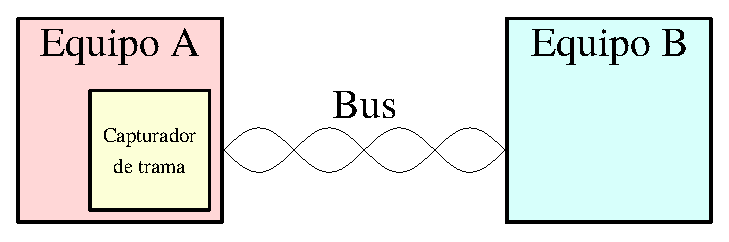
\includegraphics[width=80mm]{esquemas/esquema-captura-software.eps}
        \caption{Esquema de captura por medio de \textit{software}}
        \label{fig:captura-SW}
    \end{figure}
    
    \item \textbf{Utilizando un elemento \textit{hardware} intermedio entre los equipos (Figura~\ref{fig:captura-HW}).} \\
    Método que permite un mayor control y compatibilidad al ser totalmente independiente a los equipos implicados, pero que debido al uso de herramientas externas y a la necesidad de utilizar un equipo extra donde grabar y procesar los datos obtenidos, hace que sea un método mas laborioso, y por lo general, mas costoso.
    Se obtiene una mayor cantidad de información comparado al método \textit{software} al tener un acceso directo al propio bus.
    \begin{figure}[hbt]
        \centering
        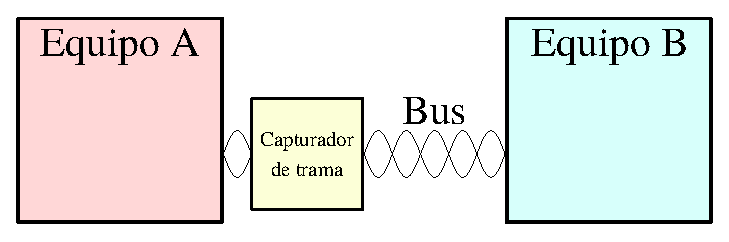
\includegraphics[width=80mm]{esquemas/esquema-captura-hardware.eps}
        \caption{Esquema de captura por medio de \textit{hardware}}
        \label{fig:captura-HW}
    \end{figure}
\end{enumerate}



\section{Sistemas \emph{software} actuales}
%* Comprobar
Debido a la gran facilidad y bajo coste que trae consigo el utilizar sistemas de captación \emph{software}, no es de extrañar que la gran mayoría de productos comerciales ya existentes se encuentran dentro de este grupo.

%* Comprobar
A continuación se muestra una lista detallada de los sistemas de captación \emph{software} más relevantes, clasificados según su tipo de licencia y ordenados según la fecha de última actualización.

%* Comprobar
\subsection{Licencia de tipo \emph{shareware}}
Se trata de \emph{software} no gratuito, de código cerrado y libre distribución entre usuarios\cite{hui2008economics}, que por lo general, posee un periodo de prueba en el que disfrutar la mayoría de las funciones sin coste. \\
Todos las aplicaciones descritas a continuación poseen una interfaz gráfica e intuitiva (Figura~\ref{fig:matriz-gui-close-sw}), y funcionan unicamente bajo al sistema operativo \emph{Windows\texttrademark}.

\begin{itemize}
    %* Comprobar
    \item \textbf{\emph{USB Monitor}\footnote{Página web del producto: \url{https://www.hhdsoftware.com/usb-monitor}} de \emph{HHD Software Ltd}.} \\
    Posee un periodo de prueba de 14 días en el que se permite utilizar todas las funciones sin restricciones. Su fecha de última actualización data del 15 de abril del 2019.

    Cabe destacar que este sistema tiene cuatro ediciones\footnote{Comparación completa de las ediciones de pago: \url{https://www.hhdsoftware.com/usb-monitor/compare}}, comentadas a continuación.
    \begin{enumerate}
        \item \textbf{Edición \emph{standard}.} \\ 
        Es la versión más básica. Incluye las siguientes funciones:
        \begin{itemize}
            \item Soporte para todas las versiones de USB.
            \item Funciones básicas de monitorización y visualizado.
            \item Filtros básicos.
            \item Guardado básico.
            \item Estadísticas de uso.
            \item Monitorización remota.
        \end{itemize}
        Su precio, a 27 de Marzo de 2019, es de 54.99\texteuro ~para uso NO comercial y 74.99\texteuro ~para uso comercial.

        \item \textbf{Edición gratuita\footnote{Se distribuye bajo el nombre de \emph{Free USB Analyzer} en: \url{https://freeusbanalyzer.com/}}.} \\
        Permite las mismas funciones que la edición \emph{standard}, limitando su uso máximo a cinco sesiones diarias, cada una de 10 minutos.
        
        \item \textbf{Edición \emph{professional}.} \\
        Incluye las ventajas de la edición \emph{standard}, añadiendo:
        \begin{itemize}
            \item Conversión de datos y visionado de datos \emph{HID}, imagen o audio, entre otros.
            \item Filtros en la captura.
            \item Capacidad de exportar los datos capturados de forma avanzada.
        \end{itemize}
        Su precio, a 27 de Marzo de 2019, es de 119.99\texteuro ~para uso NO comercial y 169.99\texteuro ~para uso comercial.
        
        \item \textbf{Edición \emph{ultimate}.} \\
        Incluye las ventajas de la edición \emph{professional}, añadiendo:
        \begin{itemize}
            \item Visor de paquetes USB en bruto.
            \item Monitorización simultanea de varios dispositivos.
            \item Scripts personalizados usando el lenguaje \emph{TypeSpript}.
        \end{itemize}
        Su precio, a 27 de Marzo de 2019, es de 159.99\texteuro ~para uso NO comercial y 224.99\texteuro ~para uso comercial.
    \end{enumerate}

    %* Comprobar
    \item \textbf{\emph{USB Sniffer}\footnote{Página web del producto: \url{https://www.eltima.com/products/usb-sniffer/}} de \emph{Eltima Software}.} \\
    \emph{Software} con 14 días de prueba, cuya versión completa tiene un precio único de mercado, a 27 de Marzo de 2019, de \$69.95 (sin incluir comisiones de cambio de divisa e impuestos). Su fecha de última actualización data del 15 de marzo del 2019.
    
    Hay que destacar las siguientes características\footnote{Lista completa de funciones: \url{https://www.eltima.com/products/usb-port-monitor\#tableCheckList}}.

    \begin{itemize}
        \item Vista completa y detallada de los datos entrantes y salientes.
        \item Soporte para \emph{HUBs} USB.
        \item Control de la captura según los datos de entrada.
        \item Soporte para todas las versiones de USB.
        \item Guardado avanzado de la trama capturada.
        \item Capacidad de marcar datos en la interfaz.
        \item Monitorización simultanea de varios dispositivos.
    \end{itemize}

    %* Comprobar
    \item \textbf{\emph{USBlyzer}\footnote{Página web del producto: \url{http://www.usblyzer.com/}}.} \\
    De manera similar que en los casos anteriores, brinda 33 días en los que probar todas la funcionalidades que ofrece sin ningún tipo de restricción. Su fecha de última actualización data del 15 de mayo del 2016.

    Caben destacar las siguientes características.

    \begin{itemize}
        \item Vista avanzada jerarquizada de todos los USB disponibles.
        \item Análisis de actividad del bus.
        \item Filtrado avanzado cuando se realizan búsquedas o capturas.
        \item Decodificación de una gran variedad de tipos de datos.
        \item Exportación avanzada.
    \end{itemize}
    El precio de una licencia, a 27 de Marzo de 2019, es de \$200 (sin incluir comisiones de cambio de divisa e impuestos), con descuentos de hasta un 46\% si se adquieren varias licencias.

    %* Comprobar
    \item \textbf{\emph{USBTrace}\footnote{Página web del producto: \url{http://www.sysnucleus.com/}} de \emph{SysNucleus}.} \\
    Igual que todos los anteriores, este programa utiliza una interfaz en la que mostrar y analizar en tiempo real el tráfico de puerto.

    Su periodo de prueba tiene una duración de 15 días, limitando además la cantidad total de la captura a 256Kb por sesión. Su fecha de última actualización data del 11 de noviembre del 2014.

    Entre otras\footnote{Lista de funciones completas: \url{http://www.sysnucleus.com/usbtrace_features.html}}, sus funciones más destacables son:
    \begin{itemize}
        \item Facilidad de uso y visualización.
        \item Variedad de filtros.
        \item Guardado avanzado.
        \item Permite análisis de los drivers utilizados por el equipo. 
        \item Captura en segundo plano.
        \item Decodificaciones personalizadas de los datos del bus.
    \end{itemize}
    Su precio unitario, a 27 de Marzo de 2019, asciende hasta \$125.00 (sin incluir comisiones de cambio de divisa e impuestos).
\end{itemize}

% \noWord[Quito las fotos??]
\begin{figure}[htbp]
    \centering
    \subfigure[\emph{USB Monitor} - \emph{HHD Software Ltd}]{
        \includegraphics[width=67mm]{analizadores_software/HHD_Software-USB_Monitor.png}
        \label{fig:matriz-gui-close-sw:hdd}
    }
    \subfigure[\emph{USB Sniffer} - \emph{Eltima Software}]{
        \includegraphics[width=67mm, height=55mm]{analizadores_software/eltima-USB_Sniffer.png}
        \label{fig:matriz-gui-close-sw:eltima}
    } \\
    \subfigure[\emph{USBlyzer}]{
        \includegraphics[width=67mm]{analizadores_software/usblyzer.png}
        \label{fig:matriz-gui-close-sw:usblyzer}
    }
    \subfigure[\emph{USBTrace} - \emph{SysNucleus}]{
        \includegraphics[width=67mm]{analizadores_software/SysNucleus-USBTrace.jpg}
        \label{fig:matriz-gui-close-sw:sysnucleus}
    }
    \caption{Interfaces gráficas de los analizadores \emph{software} de tipo \emph{shareware}. Imágenes extraídas de las páginas web de los desarrolladores.} 
    \label{fig:matriz-gui-close-sw}
\end{figure}


%* Comprobar
\subsection{Licencia de código libre}
Se trata de \emph{software} gratuito, cuyo código fuente está abiertamente disponible para su revisión y posibles modificaciones\cite{gonzalez2003introduccion}.

Dentro de este grupo hay que destacar dos herramientas, con funcionalidades similares, pero disponibles una bajo el sistema operativo \emph{Windows\texttrademark}, y la otra bajo sistemas \emph{UNIX-like}\footnote{Sistemas con comportamiento similar a sistemas Unix, sin ser necesariamente certificado a ninguna \emph{Single Unix Specification} (En español, Especificación Única Unix).}.

\begin{itemize}
    %* Comprobar
    \item \textbf{\emph{Tcpdump}\footnote{Página web del \emph{software}: \url{https://www.tcpdump.org/}}.} \\
    Herramienta bajo licencia BSD\footnote{Información detallada de la licencia: \url{https://www.tcpdump.org/license.html}}, que a través de una linea de comandos, es capaz de capturar, analizar y almacenar en un archivo PCAP paquetes de una amplia variedad de interfaces, entre las que se encuentra dispositivos \emph{USB}.

    Este método, debido a su especialización, no sería capaz de realizar un análisis detallado, por lo que sería necesario un programa adicional que posteriormente haga el estudio y clasificación de los datos de forma gráfica.

    Funciona en sistemas \emph{UNIX-like}, siempre que se tenga acceso la interfaz USB.
    
    %* Comprobar
    \item \textbf{\emph{USBPcap}\footnote{Página web del \emph{software}: \url{https://desowin.org/usbpcap/}}.} \\
    Realiza funciones similares a las que realiza \emph{Tcpdump} en cuanto a captura USB, pero funcionando bajo el Sistema Operativo Windows\texttrademark. Posee licencias GPLv2 y BSD.
    
    De igual manera que en el caso anterior, sigue siendo necesario el uso de \emph{software} de terceros para su análisis completo.
\end{itemize}

%* Comprobar
Dichos archivos generados, por lo general de tipo \emph{pcap}\cite{guyharris2015}, se pueden analizar a través de la herramienta gráfica de análisis de paquetes \emph{Wireshark}\footnote{Página web del \emph{software}: \url{https://www.wireshark.org/}} (véase figura~\ref{fig:gui-open-wireshark}). Esta está disponible para cualquiera de los dos sistemas operativos anteriores.

Hay destacar, que esta herramienta, y unicamente bajo sistemas basado en \emph{Linux}, puede ser capaz de capturar directamente y en tiempo real las tramas \emph{USB}.

\begin{figure}[hbt]
    \centering
    \includegraphics[width=125mm]{analizadores_software/wireshark.png}
    \caption{Interfaz gráfica del analizador de paquetes \emph{Wireshark}}
    \label{fig:gui-open-wireshark}
\end{figure}


%!
\section{Sistemas \emph{hardware} actuales}
En caso de que no sea posible la utilización de una captura por \emph{software}, ya sea por incompatibilidades, falta de acceso, necesidad de obtener más datos de interés o cualquier otra causa, se tendría que utilizar un sistema más complejo y costoso, por medio de \emph{hardware}.

%* Comprobar 
A continuación se muestran varios ejemplos ya existentes de este tipo, todos ellos soportan hasta la versión 2.0 de USB\cite{specification2000revision}. \\

\textit{Nota. Todos los precios de la siguiente lista, excepto que se indique, no incluyen envío, impuestos locales, o tasas de cambio de divisa.}

\begin{itemize}
    %* Comprobar 
    \item \textbf{\emph{USB Explorer 200} de \emph{Ellisys}\footnote{Página web del producto: \url{https://www.ellisys.com/products/usbex200/index.php}}.}
    
    Sistema comercial, que entre otras características\cite{ellisys2008}, destacan:
    \begin{itemize}
        \item Soporte para USB 2.0 \emph{high speed} ($480~Mbit/s$), \emph{full speed} ($12~Mbit/s$) y \emph{low speed} ($1.5~Mbit/s$).
        \item \emph{Trigger} externo de hasta 5V de entrada o 3.3V de salida.
        \item Memoria interna FIFO de $32~MBytes$.
        \item Alimentación a través de la propia conexión USB en el equipo de análisis.
        \item Dimensiones aproximadas de 150x120x65mm con un peso de 750 gramos. Véase figura~\ref{fig:ellisys-Explorer200}.
    \end{itemize}

    Aun siendo el mismo producto, este está limitado, existiendo tres variaciones, cada una con más funcionalidades y mayor precio respecto a la anterior.

    \begin{enumerate}
        \item \textbf{Edición básica.} \\
        Es la versión más básica, permitiendo unicamente capturar y posteriormente almacenar en el equipo de análisis la trama USB. \\
        Su precio, a 27 de Marzo de 2019, es de 799\texteuro.
      
        \item \textbf{Edición estándar.} \\
        Incluye las ventajas de la edición básica, añadiendo:
        \begin{itemize}
            \item Captura en tiempo real.
            \item Filtros de captura.
            \item Resumen del tráfico existente.
            \item Decodificación parcial del protocolo USB.
        \end{itemize}
        Su precio, a 27 de Marzo de 2019, es de 1599\texteuro.
        
        \item \textbf{Edición profesional.} \\
        Incluye las ventajas de la edición estándar, añadiendo:
        \begin{itemize}
            \item Decodificación completa USB.
            \item Análisis del protocolo.
            \item Capacidad de usar disparos (\emph{triggers}) externos.
        \end{itemize}
        Su precio, a 27 de Marzo de 2019, es de 3199\texteuro.
    \end{enumerate}    
    \begin{figure}[htb]
        \centering
        \includegraphics[width=50mm]{analizadores_hardware/ellisys_USBExplorer200.jpg}
        \caption{\emph{Ellisys USB Explorer 200}. Imagen extraída de la página web del fabricante.}
        \label{fig:ellisys-Explorer200}
    \end{figure}
    
    %* Comprobar
    \item \textbf{\emph{Mercury T2} de \emph{Teledyne LeCroy}\footnote{Página web del producto: \url{https://teledynelecroy.com/protocolanalyzer/usb/mercury-t2}}.}
    
    Sistema comercial, que entre otras características\cite{teledynelecroy2014}, destacan:
    \begin{itemize}
        \item Soporte para USB 2.0 \emph{high speed} ($480~Mbit/s$), \emph{full speed} ($12~Mbit/s$) y \emph{low speed} ($1.5~Mbit/s$).
        \item Memoria interna de $256~MBytes$.
        \item Almacenado automática en disco para permitir capturas de larga duración.
        \item \emph{Trigger} externo (necesario adaptador externo no incluido).
        \item Alimentación a través de la propia conexión USB en el equipo de análisis.
        \item Dimensiones aproximadas de 80x90x24mm con un peso de 158 gramos. Véase figura~\ref{fig:TeledyneLeCroy-MercuryT2}.
    \end{itemize}
    
    De igual manera que en el producto anterior, este posee varias versiones.

    \begin{enumerate}
        \item \textbf{Edición estándar.} \\
        Incluye las siguientes opciones:
        \begin{itemize}
            \item Captura y almacenaje de cualquier trama USB hasta 2.0 en tiempo real.
            \item Disparos (\emph{triggers}) para almacenar captura tanto externos, como detectando patrones en la trama.
        \end{itemize}
        Su precio, a 27 de Marzo de 2019, es de \$901.
        
        \item \textbf{Edición avanzada.} \\
        Incluye las ventajas de la edición estándar, añadiendo:
        \begin{itemize}
            \item Estadísticas en tiempo real del bus.
            \item Exportación en formato .csv.
            \item API de automatización.
        \end{itemize}
        Su precio, a 27 de Marzo de 2019, es de \$1235.
    \end{enumerate}
    \begin{figure}[htb]
        \centering
        \includegraphics[width=50mm]{analizadores_hardware/TeledyneLeCroy_MercuryT2.jpg}
        \caption{\emph{Teledyne LeCroy Mercury T2}. Imagen extraída de la página web del fabricante.}
        \label{fig:TeledyneLeCroy-MercuryT2}
    \end{figure}

    %* Comprobar
    \item \textbf{\emph{Beagle USB} de \emph{Total Phase}\footnote{Página web del producto: \url{https://www.totalphase.com/protocols/usb/}}.}
    
    Dentro de la amplia gama de productos que disponen, hay dos que destacan principalmente.
    \begin{enumerate}
        \item \textbf{\emph{Beagle USB 480}\cite{totalphase12-2018}.}
        De todas las versiones que poseen, esta es la más básica que permite hasta capturas \emph{high speed} de ($480~Mbit/s$).
        \begin{itemize}
            \item Captura en tiempo real.
            \item Estadísticas en tiempo real.
            \item $64MBytes$ de memoria integrada.
            \item \emph{Triggers} externos de entrada y salida.
            \item Sincronización básica.
            \item API de control.
        \end{itemize}
        Su precio, a 27 de Marzo de 2019, es de \$2250.
        
        \item \textbf{\emph{Beagle USB 480 Power}\cite{totalphase480-2018} - Edición estándar.} \\
        Posee las mismas ventajas que el producto anterior, pero aumentando la memoria integrada de $64MBytes$ a $256MBytes$ y añadiendo capacidad de medir la tensión y corriente del propio Bus.\\
        Su precio, a 27 de Marzo de 2019, es de \$1599.
        
        \item \textbf{\emph{Beagle USB 480 Power}\cite{totalphase480-2018} - Edición \emph{ultimate}.} \\
        Mejora las capacidades de disparos (\emph{triggers}) respecto a la versión estándar.\\
        Su precio, a 27 de Marzo de 2019, es de \$2950.
    
        \begin{figure}[htbp]
            \centering
            \subfigure[\emph{Beagle USB 480}]
            {
                \includegraphics[width=40mm]{analizadores_hardware/TotalPhase_beagle480.jpg}
                \label{fig:TotalPhase-480}
            }
            \subfigure[\emph{Beagle USB 480 Power}]{
                \includegraphics[width=40mm]{analizadores_hardware/TotalPhase_beagle480Power.jpg}
                \label{fig:TotalPhase-480Power}
                }
            \caption{Productos de \emph{Total Phase}. Imágenes extraídas de la página web del fabricante.} 
            \label{fig:TotalPhase}
        \end{figure}
    \end{enumerate}
    
    %* Comprobar
    \item \textbf{\emph{USB Sniffer}\footnote{Página web del proyecto: \url{http://ultra-embedded.com/usb_sniffer/}} de \emph{Ultra-Embedded}}

    Proyecto NO comercial, que usando una \emph{FPGA Xilinx Spartan 6 LX9}, y una placa de desarrollo encargada de procesar la capa física, es capaz de capturar hasta USB 2.0 \emph{high speed} ($480~Mbit/s$). En la figura~\ref{fig:ultra-embedded} se muestra una imagen del proyecto.
    
    Al ser un proyecto personal, no dispone de un producto final que se pueda adquirir, por lo que si se quiere utilizar se deben comprar las piezas por separado. Además, el código utilizado es \emph{open source}, por lo que se puede replicar sin ningún tipo de problema. Su precio aproximado se muestra en la tabla~\ref{tab:precio-ultra-embedded}.

    \begin{table}[hbtp]
        \centering
        \caption{Componentes y precio de la propuesta de analizador USB de \emph{Ultra-Embedded}}
        \label{tab:precio-ultra-embedded}
        \begin{tabular}{|c|c|c|}
            \hline
            \textbf{Componente} &
            \textbf{Unidades} &
            \textbf{Precio} \\ \hline
            \hline

            FPGA Xilinx Spartan 6 LX9 &
            1 & \$75 \\ \hline

            Placa de desarrollo USB3300 &
            1 &
            \$8 \\ \hline

            Cable IDC &
            1 &
            \$5 \\ \hline
            
            \multicolumn{1}{r}{} &
            \multicolumn{1}{c}{Precio total:} &
            \multicolumn{1}{c}{\$88} \\
        \end{tabular}
    \end{table}

    \begin{figure}[hbtp]
        \centering
        \includegraphics[width=85mm]{analizadores_hardware/Ultra-Embedded.jpg}
        \caption{\emph{USB Sniffer}. Imagen extraída de la página web del proyecto.}
        \label{fig:ultra-embedded}
    \end{figure}
\end{itemize}


\newpage
%* Comprobar
\section{Comparativa de sistemas \emph{software}}
%* Comprobar
En la tabla~\ref{tab:comparacion-sw} se muestra una comparativa de los productos de captura \emph{software} más destacados.

Se aprecia, que dentro del \emph{software} de pago, el que más funcionalidades ofrece a razón de su precio, es \emph{USB Sniffer} de \emph{Eltima Software}, seguido de \emph{USB Monitor} de \emph{HHD Software Ltd}. Las otras dos opciones no poseen actualizaciones recientes, y su precio es más elevado, por lo que son menos recomendables.

Por otro lado, las opciones de \emph{código libre}, aun teniendo una curva de aprendizaje muy superior, son opciones totalmente viables y recomendables.

%* Comprobar
\begin{table}[!hbtp]
    \centering
    \caption{Comparativa de sistemas \emph{software}}
    \label{tab:comparacion-sw}
    \begin{tabular}{|c|c|c|c|c|}
        \hline
        Nombre &
        \begin{tabular} {@{}c@{}}
            Licencia y \\ precio
        \end{tabular} &
        Ventajas &
        Desventajas \\ \hline
        \hline
        
        \begin{tabular}
            {@{}c@{}} \textbf{\emph{USB Monitor}} de \\ \emph{HHD Software Ltd}
        \end{tabular} &
        \begin{tabular} {@{}c@{}}
            \emph{Shareware} \\ Desde 54.99\texteuro
        \end{tabular} &
        \begin{tabular} {@{}c@{}}
            Actualizaciones frecuentes. \\
            Decodificación \enquote{en vivo}. \\
            Gran sencillez de uso. \\
            Posee versión gratuita. \\
        \end{tabular} &
        \begin{tabular} {@{}c@{}}
            Extra para uso comercial.  \\
            Varias ediciones. \\
        \end{tabular} \\ \hline
        
        \begin{tabular}
            {@{}c@{}} \textbf{\emph{USB Sniffer}} de \\ \emph{Eltima Software}
        \end{tabular} &
        \begin{tabular} {@{}c@{}}
            \emph{Shareware} \\ \$69.95
        \end{tabular} &
        \begin{tabular} {@{}c@{}}
            Monitorización simultanea. \\
            Soporte para \emph{HUBs} USB. \\
            Gran sencillez de uso. \\
        \end{tabular} &
        \begin{tabular} {@{}c@{}}
            Sin capacidad de decodificación. \\
        \end{tabular} \\ \hline
        
        \textbf{\emph{USBlyzer}} &
        \begin{tabular} {@{}c@{}}
            \emph{Shareware} \\ Hasta \$200
        \end{tabular} &
        \begin{tabular} {@{}c@{}}
            Decodificación incluida. \\
            Exportación avanzada.  \\
        \end{tabular} &
        \begin{tabular} {@{}c@{}}
            Sin actualizaciones recientes. \\
            Precio elevado. \\
        \end{tabular} \\ \hline
        
        \begin{tabular}
            {@{}c@{}} \textbf{\emph{USBTrace}} de \\ \emph{SysNucleus}
        \end{tabular} &
        \begin{tabular} {@{}c@{}}
            \emph{Shareware} \\ \$125.00
        \end{tabular} &
        \begin{tabular} {@{}c@{}}
            Decodificado personalizado. \\
            Análisis de \emph{drivers}. \\
        \end{tabular} &
        \begin{tabular} {@{}c@{}}
            Sin actualizaciones recientes. \\
            Pocas funcionalidades. \\
        \end{tabular} \\ \hline
        
        \begin{tabular}
            {@{}c@{}} \textbf{\emph{Tcpdump}} y \\ \textbf{\emph{USBPcap}}
        \end{tabular} &
        \begin{tabular} {@{}c@{}}
            \emph{Código libre} \\ --
        \end{tabular} &
        \begin{tabular} {@{}c@{}}
            Soporte de la comunidad. \\
            Multiplataforma. \\
            Gratuito. \\
        \end{tabular} &
        \begin{tabular} {@{}c@{}}
            Solo realiza capturas de trama. \\
            Pocas funcionalidades extra. \\
            Sin interfaz gráfica. \\
        \end{tabular} \\ \hline
        
        \textbf{\emph{Wireshark}} &
        \begin{tabular} {@{}c@{}}
            \emph{Código libre} \\ --
        \end{tabular} &
        \begin{tabular} {@{}c@{}}
            Variedad de funcionalidades. \\
            Filtrado avanzado. \\
            Multiplataforma. \\
            Gratuito. \\
        \end{tabular} &
        \begin{tabular} {@{}c@{}}
            No realiza capturas. \\
            Poco intuitivo. \\
        \end{tabular} \\ \hline
    \end{tabular}
\end{table}


%* Comprobar
\section{Comparativa de sistemas \emph{hardware}}
%* Comprobar
En la tabla~\ref{tab:comparacion-hw} se muestra una comparativa de los productos de captura \emph{hardware} más destacados.

Se aprecia que dentro de este grupo, el equipo más recomendable a razón de sun funcionalidades ofrecidas y precio es el \emph{Mercury T2} de \emph{Teledyne LeCroy}. Si se buscan más funciones y almacenamiento es más viable utilizar el  {\emph{Beagle USB 480 Power} de \emph{Total Phase}.

%* Comprobar
\begin{table}[!hbtp]
    \centering
    \caption{Comparativa de sistemas \emph{hardware}}
    \label{tab:comparacion-hw}
    \begin{tabular}{|c|c|c|c|c|}
        \hline
        Nombre &
        \begin{tabular} {@{}c@{}}
            Licencia y \\ precio
        \end{tabular} &
        Ventajas &
        Desventajas \\ \hline
        \hline
        
        \begin{tabular}
            {@{}c@{}} \textbf{\emph{USB Explorer 200}} de \\ \emph{Ellisys}
        \end{tabular} &
        \begin{tabular} {@{}c@{}}
            Cerrado. \\ Desde 799\texteuro \\ a 3199\texteuro
        \end{tabular} &
        \begin{tabular} {@{}c@{}}
            Posibilidad de análisis completo. \\
            Captura en tiempo real. \\
            Disparos externos. \\
        \end{tabular} &
        \begin{tabular} {@{}c@{}}
            Versión básica simple. \\
            Escasa memoria. \\
            Sistema costoso. \\
        \end{tabular} \\ \hline
        
        \begin{tabular}
            {@{}c@{}} \textbf{\emph{Mercury T2}} de \\ \emph{Teledyne LeCroy}
        \end{tabular} &
        \begin{tabular} {@{}c@{}}
            Cerrado. \\ Desde \$901 \\ a \$1235
        \end{tabular} &
        \begin{tabular} {@{}c@{}}
            API de automatización. \\
            Disparos avanzados. \\
            Tamaño reducido. \\
        \end{tabular} &
        \begin{tabular} {@{}c@{}}
            Adaptador para disparos \\ externos no incluido. \\
            Pocas funciones extras. \\
        \end{tabular} \\ \hline
        
        \begin{tabular}
            {@{}c@{}} \textbf{\emph{Beagle USB 480}} de \\ \emph{Total Phase}
        \end{tabular} &
        \begin{tabular} {@{}c@{}}
            Cerrado. \\ \$2250
        \end{tabular} &
        \begin{tabular} {@{}c@{}}
            Estadisticas en tiempor real. \\
            API de automatización. \\
            Sincronización básica. \\
        \end{tabular} &
        \begin{tabular} {@{}c@{}}
            Sin funciones de analisis. \\
            Escasa memoria. \\
        \end{tabular} \\ \hline
        
        \begin{tabular}
            {@{}c@{}} \textbf{\emph{Beagle USB 480 Power}} de \\ \emph{Total Phase}
        \end{tabular} &
        \begin{tabular} {@{}c@{}}
            Cerrado. \\ Desde \$1599 \\ a \$2950
        \end{tabular} &
        \begin{tabular} {@{}c@{}}
            Alta capacidad de memoria. \\
            Analisis de potencia. \\
        \end{tabular} &
        \begin{tabular} {@{}c@{}}
            Versión estándar sin \\disparos avanzados. \\
        \end{tabular} \\ \hline
        
        \begin{tabular}
            {@{}c@{}} \textbf{\emph{USB Sniffer}} de \\ \emph{Ultra-Embedded}
        \end{tabular} &
        \begin{tabular} {@{}c@{}}
            Código libre. \\ Aporx. \$88
        \end{tabular} &
        \begin{tabular} {@{}c@{}}
            Muy económico. \\
            Código libre. \\
        \end{tabular} &
        \begin{tabular} {@{}c@{}}
            No está en venta directa. \\
            Solo permite captura. \\
            Memoria escasa. \\
        \end{tabular} \\ \hline
    \end{tabular}
\end{table}



% \chapter{Motivación y antecedentes}
% \label{ch:antecedentes_plantilla}

% El problema que pretendes resolver está dentro de un contexto que el cliente debe conocer.  Esta sección aporta información para conocer en detalle la importancia del problema y la dificultad para resolverlo con los productos y programas disponibles actualmente.

% Este capítulo concentrará el grueso de las citas del TFG.  Dado que se trata del primer trabajo profesional, el alumno no suele estar familiarizado con las citas bibliográficas.  Pon toda tu atención en qué citas y cómo lo citas.  Revisa la sección~\ref{sec:bibliografia-citas} para las reglas mínimas que deben cumplir las citas.

% \warning{Es muy importante respetar la regla de atribuir correctamente.  No es aceptable desde el punto de vista legal, ni tampoco desde el punto de vista ético, copiar trabajo de otros sin atribuirlo correctamente a los autores.}

% Esta sección debe estudiar de forma sistemática todas las opciones ya disponibles en la actualidad para resolver el problema. No basta con una mera enumeración, hay que estudiarlos mínimamente para explicar por qué no son una solución para el problema o qué podría aportar a la solución del problema.

% Un método sistemático para realizar esta parte del TFG es la revisión sistemática de literatura, conocida habitualmente por sus siglas en inglés SLR (\emph{Sistematic Literature Review}).  Un resumen muy sencillo de cómo realizar una SLR puede encontrarse en~\cite{anderskofodpetersen2014}.  También encontrarás consejos prácticos en~\cite{sandroschulze2017}.  Para un proceso más detallado, especialmente si tu problema tiene mucho arte previo, puedes consultar~\cite{barbarakitchenhamstuartcharters2007}.  Si no hay mucho arte previo pon este capítulo y el siguiente juntos.

% En una tesis doctoral el análisis sistemático del estado del arte es esencial. En un TFG es importante, pero no hay que perder la cabeza.  Un TFG son unas 300 horas de trabajo de un estudiante medio que ya posea los conocimientos generales necesarios (volveremos a esto más tarde).  Considero que un buen análisis del estado del arte corresponde a un trabajo de entre 25 horas y 100 horas, dependiendo del tema del proyecto.  Si el tema es muy específico es más fácil hacer el estudio del estado del arte.

% Termina este capítulo con una sección que resuma el estado del arte e identifique las lagunas lo más claramente posible.  Una tabla comparativa o un gráfico pueden ser formas interesantes de presentar la información.